\chapter{Introdução}
\label{chap:Chapter1}
Atualmente, num mercado crescentemente competitivo e exigente, a necessidade de inovar, de obter vantagem competitiva e simultaneamente, tornar os processos industriais simples e altamente eficazes, recorrendo às tecnologias mais atuais, abrem caminho a uma nova mudança. O fenómeno da Indústria 4.0 surge como a nova (quarta) revolução industrial, baseando-se nas mais recentes tecnologias, que incluem os sistemas ciber-físicos, a \gls{iot} e a \gls{ios}, as quais se baseiam na comunicação através da Internet, permitindo uma interação contínua e partilha de informação entre humanos, entre máquinas e entre o ser humano e máquina~\parencite{complex_view_industry40}. 

A Indústria 4.0 assenta numa variedade de conceitos fundamentais, de diferentes áreas de conhecimento, nomeadamente a noção de \textit{Smart Factory\footnote{Fábrica Inteligente, equipada com sensores, atuadores e sistemas autónomos, permitindo assim um controlo autónomo de processo.}}, a capacidade de auto-organização, através da descentralização dos sistemas produtivos, e a interação entre o mundo físico e o digital~\parencite[Fundamental Concepts, p.240]{industry40}. No entanto, é a capacidade de adaptação à necessidade humana, principalmente a \gls{ihc}, que se pretende explorar com presente trabalho.

Segundo~\textcite[p.1]{natural_language_translation_intersaction_ai_hci}~\inquotes{as áreas de \gls{ia} e Interação Humano-Computador (\gls{ihc}) estão, cada vez mais, a influenciar-se mutuamente. Sistemas amplamente usados como o Google Translate, Facebook Graph Search e RelateIQ escondem a complexidade de sistemas de larga escala de \gls{ia} através de interfaces intuitivas.}\footnote{Tradução livre do autor. No original~\inquotes{The fields of artificial intelligence (AI) and human-computer interaction (HCI) are influencing each other like never before. Widely used systems such as Google Translate, Facebook Graph Search, and RelateIQ hide the complexity of large-scale AI systems behind intuitive interfaces.}.}. Apesar de terem propósitos diferentes, ambas as áreas se complementam, na medida em que se focam na relação entre ser humano e máquina. Se a \gls{ia} tem como objetivo emular o intelecto humano, já a \gls{ihc} foca-se em abordagens empíricas de usabilidade e fatores humanos, que influenciam a forma como os utilizadores interagem com o computador~\parencite{natural_language_translation_intersaction_ai_hci}. 

A capacidade dum sistema interpretar a linguagem dos seres humanos e apresentar a informação de uma forma adequada, principalmente no contexto da Indústria 4.0, destaca-se como um fator impulsionador da adaptabilidade do mundo digital à necessidade humana. Nesse sentido, a área de \gls{pln}, a qual se debruça na capacidade dos computadores \inquotes{entenderem} a linguagem humana~\parencite[p.1]{applied_natural_language_processing_with_python}, permite construir ferramentas capazes de definir ações, extrair conhecimento dum sistema e apresentá-lo num formato adequado, a partir de conteúdo textual especificado pelo utilizador, de acordo com a sua própria linguagem. 

% Enunciado do problema
\section{Problema}
\label{sec:chap01_problem}
O conceito de \gls{mes}, um sistema que, além de gerir as operações dum determinado processo fabril, mantém dados relativos às diversas etapas inerentes ao processo em questão, está intrinsecamente relacionado com a Indústria 4.0, uma iniciativa que se destina a criar fábricas inteligentes, usando tecnologias como os \glspl{cps}, a \gls{iot} e \textit{Cloud Computing}~\parencite{intelligent_manufacturing_context_industry40_review}. O {\productname} é um destes sistemas. Contudo, a capacidade de adaptação às características dos utilizador é um requisito complexo, que nem sempre é passível de ser cumprido. Isso pode tornar o produto difícil de usar, numa perspetiva de acesso a informação relevante para o processo e de apoio à decisão. Por outras palavras, se o utilizador pretende efetuar uma determinada pesquisa, necessita de conhecer os detalhes da ferramenta a usar, ao invés de simplesmente \inquotes{pedir} (através de texto ou voz) ao sistema que lhe devolva o resultado.

\textbf{A conceção de um módulo de linguagem natural para interface com o {\productname}, permitindo a consulta e pesquisa de estados do processo de fabrico}, torna-se importante para o sistema, uma vez que possibilita o utilizador interagir com o sistema de uma forma simples, intuitiva, eficiente e natural, através de escrita.

% Objetivos
\section{Objetivos}
\label{sec:chap01_objectives}
De uma maneira geral, com este trabalho pretende-se desenvolver um protótipo, cuja abordagem pode ser usada para solução final baseada em linguagem natural, que promova a interação do utilizador com o sistema \gls{mes}. Com o intuito de solucionar o problema enunciado na Secção~\ref{sec:chap01_problem}, definem-se os seguintes objetivos:

\begin{enumerate}
    \item
    {
        \textit{Contextualizar o problema numa perspetiva de negócio} -- análise detalhada do problema, as implicações que tem para negócio e para o produto \gls{mes}, descrevendo o valor intrínseco à solução (Capítulo~\ref{chap:Chapter2});
    }
    \item
    {
        \textit{Estudar soluções disponíveis no mercado e/ou ferramentas de processamento de linguagem natural} -- obtenção de informação da área de conhecimento envolvida, de soluções semelhantes e de ferramentas tipicamente usadas na implementação de tais módulos (Capítulo~\ref{chap:Chapter3});
    }
    \item
    {
        \textit{Definir a abordagem mais adequada, considerando as diversas opções apresentadas} -- comparação e avaliação das diversas opções identificadas (Capítulo~\ref{chap:Chapter3});
    }
    \item
    {
        \textit{Especificação da arquitetura do módulo} -- que permita responder aos requisitos definidos e antecipar soluções para possíveis problemas;
    }
    \item
    {
        \textit{Descrever a semântica de domínio} -- identificação dos domínios a explorar e construção de uma base de conhecimento semântico para o módulo;
    }
    \item
    {
        \textit{Desenvolvimento de prova de conceito} -- implementação do protótipo de acordo com a arquitetura conceptualizada;
    }
    \item
    {
        \textit{Prover o protótipo de um mecanismo de feedback para auto-aprendizagem} -- o que permitirá ao módulo adaptar-se às necessidades do utilizador, melhorando a qualidade das suas respostas. Numa fase inicial, este mecanismo pode não constar no protótipo, ou pode consistir em simplesmente questionar o utilizador sobre a exatidão da resposta apresentada;
    }
    \item
    {
        \textit{Avaliar a qualidade da solução desenvolvida} -- com base na hipótese formulada em~\ref{sec:chap01_hypothesis} e na estratégia de avaliação definida em~\ref{enum:chap01_qualitystrategies}, concluir acerca da qualidade da abordagem seguida e do contributo do trabalho para a resolução do problema.
    }
\end{enumerate}

% Âmbito
\section{Âmbito}
\label{sec:chap01_scope}
Embora os objetivos estejam definidos, surge a necessidade de explicitar sucintamente o âmbito deste trabalho, bem como os pressupostos a ter em consideração. Por conseguinte, os seguintes assuntos serão abordados:

\begin{itemize}
    \item
    {
        A contextualização do problema da empresa com a prova de conceito a ser desenvolvida, o seu enquadramento com a Indústria 4.0 e utilidade para o cliente final; 
    }
    \item 
    {
        Os conceitos teóricos e adversidades inerentes ao problema, ainda que explorados de uma forma genérica, evitando abordar pormenores ou especificidades do tema;
    }
    \item
    {
        A apresentação e explicação dos exemplos de resolução de problemas semelhantes por parte de terceiros, fazendo um levantamento das características relevantes para este projeto;
    }
    \item
    {
        As ferramentas disponíveis e relevantes para este contexto, passíveis de ser aplicadas nesta prova de conceito;
    }
    \item
    {
        O método científico e processo de engenharia adotado na busca duma abordagem para resolução do problema em questão.
    }
\end{itemize}

Por outro lado, alguns tópicos são demasiado amplos para serem explorados, ou simplesmente não se enquadram nos objetivos desta tese, pelo que não serão abordados:

\begin{itemize}
    \item
    {
        O enquadramento do problema com outros \glspl{mes}. Apenas é contemplada a realidade do problema no contexto do {\productname};
    }
    \item
    {
        As soluções e ferramentas de linguagem natural que não mostrem evidências de relevância para o problema, tendo em conta os critérios de preço, adesão da comunidade de desenvolvimento e respetiva complexidade;
    }
    \item 
    {
        A inclusão de diferentes domínios na solução desenvolvida.
    }
\end{itemize}

O termo \inquotes{Domínio} é empregue ao longo do texto para denotar um conjunto de características que descrevem uma família de conceitos comuns a um determinado processo. Por exemplo, duas empresas que produzem equipamentos médicos, apesar de poderem ter processos de fabrico diferentes, abordam o mesmo domínio.

Neste trabalho assume-se que a solução a desenvolver, embora desejada para integrar em diferentes processos de manufatura, é uma prova de conceito, pelo que deverá considerar um domínio específico e consequentemente, lidar com a semântica específica desse domínio.

% Avaliação da solução
\section{Avaliação e Experimentação}
\label{sec:chap01_solutionevaluation}
A avaliação do resultado final é imprescindível para a concluir acerca do sucesso do presente trabalho, permitindo perceber se a conjetura fundada a respeito da prova de conceito é aceite. Desse modo, formula-se a hipótese colocada para a abordagem escolhida, a respetiva metodologia de avaliação e experimentação e os critérios de sucesso a serem considerados.

\subsection{Formulação das Hipóteses}
\label{sec:chap01_hypothesis}
Para a resolução do problema da empresa explicitado em~\ref{sec:chap01_problem}, o qual foca a melhoria da interação do {\productname} com o utilizador, surgem as seguintes questões:

\begin{enumerate}
    \item
    {
        A integração de um módulo de linguagem natural pode, de facto, melhorar a usabilidade do produto e consequentemente, simplificar processo de apoio à decisão?
    }
    \item
    {
        De que forma se pode avaliar a adequabilidade das respostas da solução às necessidades básicas dos utilizadores?
    }
\end{enumerate}

Embora as perguntas anteriores sejam relevantes para a formulação de hipóteses para a solução final, e devem ser tidas em consideração na abordagem escolhida, não terão um peso significativo na avaliação do resultado deste trabalho. O foco desta tese, tal como descrito na Secção~\ref{sec:chap01_objectives}, é o desenvolvimento de um protótipo, em que a abordagem pode ser seguida para a implementação de uma solução definitiva no {\productname}. Assim, surge outra pergunta mais pertinente para esta fase e respetiva hipótese:

\begin{itemize}
    \item
    {  
        \textit{Questão} -- Qual a abordagem adequada para a tradução de linguagem natural numa linguagem capaz de extrair conhecimento de armazéns de dados?
    }
    \item
    {
        \textit{Hipótese} -- A abordagem escolhida permite a extração de conhecimento de armazéns de dados a partir de linguagem natural.
    }
\end{itemize}

A hipótese apresentada auxilia na definição da metodologia de avaliação a adotar na presente tese. A refutação ou aceitação da hipótese formulada permite concluir acerca do trabalho realizado, e da necessidade de reformulação ou adoção de novas hipóteses.

\subsection{Metodologia de Avaliação}
\label{sec:chap01_evaluationmethodologies}
Com o propósito de perceber se a abordagem tomada no protótipo desenvolvido é adequado para o {\productname} e para o utilizador final, e levando em consideração a hipótese formulada anteriormente, definem-se as seguintes estratégias para a metodologia de avaliação deste trabalho:

\begin{enumerate}
\label{enum:chap01_qualitystrategies}
    \item 
    {
        \textit{Garantir que a solução analisa e responde corretamente a um conjunto de perguntas pré-definidas} -- a solução deverá responder adequadamente a um conjunto limitado de perguntas:
        \begin{itemize}
            \item 
            {
                Quantas operações $O$ foram executadas por semana, durante o mês $M$?
            }
            \item
            {
                Qual o número de operações $O$ por produto e turno, durante o mês $M$?
            }
            \item
            {
                Qual a média de $X$ de operações $O$, no passo $P$ do processo, por turno, no mês $M$? 
            }
            \item
            {
                Qual o número de materiais cujo valor de $X$ é inferior a $Y$, para o passo $P$ do processo, agrupando por $G$?
            }
        \end{itemize}
        
        Nas questões apresentadas, as letras representam as variáveis inerentes ao domínio, que o utilizador conhece e que o sistema deve ser capaz de reconhecer.
    }
    \item
    {
        \textit{Usar as respostas devolvidas pelo protótipo para concluir acerca da sua exatidão} -- as respostas fornecidas pelo protótipo, face à resposta expectável, permitirão perceber se a abordagem seguida é adequada.
    }
\end{enumerate}

Ambas estratégias possibilitam perceber a adequabilidade da abordagem para solução a ser integrada no produto e para o utilizador, quer numa perspetiva de facilidade de utilização, quer na exatidão da resposta dada.

\subsection{Critérios de Sucesso}
De seguida, enumeram-se os critérios de sucesso para o trabalho:

\begin{enumerate}
    \item 
    {
        \textit{A hipótese apresentada anteriormente é aceite} -- a abordagem escolhida apresenta resultados satisfatórios face à metodologia de avaliação definida para este trabalho;
    }
    \item
    {
        \textit{A abordagem apresentada é extensível e de fácil integração no {\productname}} -- garante-se que a arquitetura especificada considerou a existência de diversos domínios, facilidade e capacidade de integração com o produto;
    }
    \item
    {
        \textit{Prova de conceito dá resposta correta às questões que lhe são colocadas} -- que implica responder corretamente às questões listadas em~\ref{enum:chap01_qualitystrategies}, garantindo que a resposta fornecida é semelhante ou igual à resposta que seria esperada;
    }
    \item
    {
        \textit{A abordagem é adotada ou refinada de forma a que possa ser usada na solução final} -- a abordagem revela-se efetiva na resolução do problema, e com o levantamento de possíveis melhorias, pode ser implementada no {\productname}.
    }
    % \item 
    % {
    %     \textit{Tese escrita} -- na qual se abordam o problema, o contexto no qual se insere e o valor que traz ao produto final. Deve conter o estado da arte, apresentando a revisão da literatura existente, focando nas soluções semelhantes e/ou ferramentas relevantes que perspetivam estratégias de solução para o problema. Por fim, descreve-se a solução proposta, contemplando cada uma das fases inerentes ao seu desenvolvimento (visão, análise, desenho e implementação) e faz-se a conclusão acerca do trabalho (todos os objetivos descritos em~\ref{sec:chap01_objectives});
    % }
\end{enumerate}

% Contribuições
\subsection{Contribuições}
\label{sec:chap01_contributions}
O trabalho a ser desenvolvido pretende providenciar uma solução para o problema descrito anteriormente (Secção \ref{sec:chap01_problem}). Não se aspira fornecer uma solução definitiva, espera-se sim, contribuir com conhecimento de carácter teórico e prático (\idest{um protótipo}), que possibilite a integração futura de uma nova funcionalidade num produto já existente, trazendo-lhe mais-valia funcional, destacando-o dos seus concorrentes. No decorrer deste trabalho serão abordados temas relativos a \gls{mes}, a \gls{ia}, especificamente \gls{pln}, e \textit{Business Intelligence}.

Resumidamente, as contribuições esperadas são a seguir enunciadas:

\begin{itemize}
    \item
    {
        Estado da arte no domínio de Processamento de Linguagem Natural, aplicadas à conversão de texto para \gls{sql} e sistemas análogos à solução a desenvolver;
    }
    \item 
    {
        Documentação dos requisitos de sistema, incluindo análise e desenho, constando os respetivos artefactos de \gls{uml};
    }
    \item 
    {
        Dicionário semântico do domínio a ser definido para o módulo;
    }
    \item
    {
        Especificação e desenvolvimento do protótipo, considerando a futura integração com o sistema {\productname};
    }
    \item
    {
        Conceção do mecanismo de \textit{feedback} permitindo a adaptação ao utilizador e consequentemente, a auto-aprendizagem do sistema.
    }
\end{itemize}

De uma forma geral, é realçada a contribuição para o avanço do conhecimento no domínio da \gls{ia}, mais especificamente na área da \gls{pln}, aplicada ao contexto dos sistemas \gls{mes} e que servirá como base para a integração duma solução deste tipo no {\productname}.

% Plano e Método de Trabalho
\section{Plano e Método de Trabalho}
\label{sec:chap01_workmethodology}

Um plano de trabalho é uma ferramenta importante na gestão de qualquer projeto, na medida em que permite ter visibilidade da sua extensão temporal, das tarefas a realizar e do período associado a cada uma delas. Na Figura~\ref{fig:planning-gantt_chart} demonstra-se o diagrama de \textit{Gantt}, contendo as tarefas inerentes a cada uma das fases do projeto, descriminadas na tabela abaixo.

\begin{table}[!ht]
\caption{Fases do projeto, periodicidade e respetiva duração}
\label{tab:project-phases}
\centering
\resizebox{\textwidth}{!}{\begin{tabular}{l|l|l|l}
%
\toprule
%
\tabhead{Fase do Projeto}&\tabhead{Data Prevista de Início}&\tabhead{Data Prevista de Fim}&\tabhead{Duração (dias)}\\ 
%
\midrule
Conceção                 & 01-Jan-2019                      & 16-Fev-2019                   & 46                      \\
Análise                  & 11-Fev-2019                      & 08-Março 2019                 & 25                      \\
Desenvolvimento          & 04-Março-2019                    & 17-Maio-2019                  & 74                      \\
Validação                & 17-Maio-2019                     & 12-Junho-2019                 & 26                      \\
Documentação             & 01-Jan-2019                      & 30-Junho-2019                 & 180                     \\ 
%
\bottomrule
\end{tabular}}
\end{table}

A Tabela~\ref{tab:project-phases} carece de informação sucinta de cada uma das fases, pelo que se passam a descrever:

\begin{itemize}
    \item
    {
        \textit{Conceção} -- engloba as tarefas que relacionadas com o problema, o seu enquadramento, o estudo do valor e estado da arte. Ou seja, a visão do projeto;
    }
    \item
    {
        \textit{Análise} -- nesta fase, faz-se o levantamento dos requisitos, a escolha e definição da semântica de domínio, estipulam-se a(s) tecnologia(s) a utilizar e especifica-se a arquitetura para o módulo. A presente fase consiste no estudo e preparação para o desenho da solução; 
    }
    \item
    {
        \textit{Desenvolvimento} -- desenvolve-se a solução conjeturada na fase anterior, envolvendo um período de experimentação de código base da arquitetura definida (para possível reestruturação ou ajuste);
    }
    \item
    {
        \textit{Validação} -- avalia-se a solução com base nos critérios definidos na secção~\ref{sec:chap01_solutionevaluation} e consequentemente, podem-se registar melhorias para o módulo. É nesta fase que também se demonstra a solução às partes interessadas do trabalho (\exempligratia{\gls{ceo}, \gls{cto}, {\supname}, orientador do projeto, {\cosupname}, responsável pelo projeto etc.});
    }
    \item
    {
        \textit{Documentação} -- engloba a escrita da tese como veículo de transmissão de conhecimento obtido e de outros documentos de suporte, a serem usados no contexto empresarial (\exempligratia{documento de especificação de requisitos de \textit{software}, especificação arquitetural de \textit{software}, manual de instalação e outros que façam sentido}).
    }
\end{itemize}

Quanto ao método de trabalho a seguir na realização deste trabalho, são considerados os seguintes passos:

\begin{enumerate}
    \item 
    {
        \textit{Revisão de literatura disponível sobre o contexto do problema} -- com o objetivo de perceber o estado atual do {\productname} e as implicações que o módulo trará, assim como concluir acerca do valor da solução para o produto;
    }
    \item
    {
        \textit{Revisão de literatura existente acerca de \gls{pln} e paradigmas arquiteturais relacionados} -- adquirir conhecimentos sobre técnicas e ferramentas de \gls{pln}, principalmente analisando soluções já existentes, identificando aspetos relevantes para o trabalho e outros que não foram contemplados;
    }
    \item
    {
        \textit{Idealização do módulo} -- depois da análise dos conhecimentos adquiridos com as revisões realizadas nos passos descritos anteriormente, parte-se para o levantamento dos requisitos junto das partes interessadas do projeto, resultando na concepção de um módulo capaz de lhes dar resposta; 
    }
    \item
    {
        \textit{Estudo do domínio de negócio} -- com o intuito de entender a semântica do negócio em questão e definir um dicionário a ser usado pela solução;
    }
    \item
    {
        \textit{Implementação do módulo e validação} -- o foco é pôr em prática a solução conceptualizada nas fases anteriores. Após a implementação, são realizam-se testes com vista a perceber se os resultados obtidos são os esperados e proceder às melhorias que forem evidentes;
    }
    \item
    {
        \textit{Elaboração da documentação} --  por fim, passa-se à escrita do presente documento e de documentos de suporte, baseando-se nas observações, nas experiências e conclusões obtidas ao longo do projeto.
    }
\end{enumerate}

\clearpage
\begin{sidewaysfigure}[!ht]
    \centering
    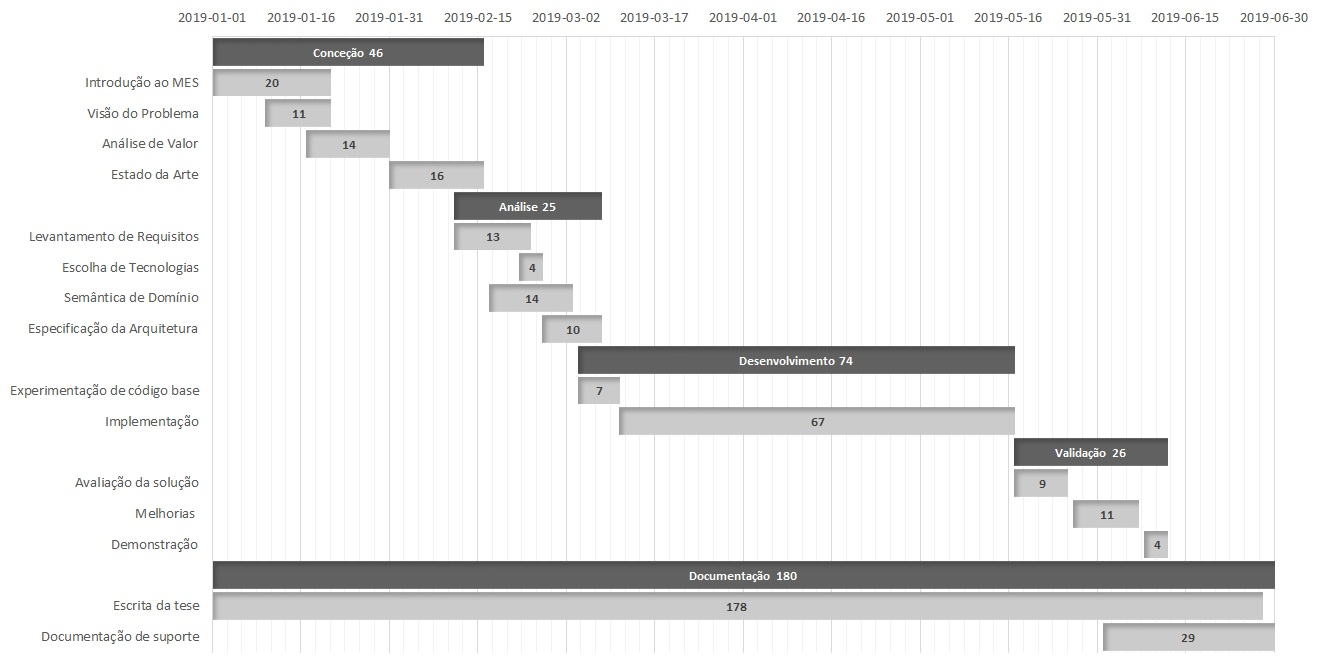
\includegraphics[width=1.0\textwidth]{ch01/assets/gantt.jpg}
    \caption{Diagrama de \textit{Gantt} referente ao planeamento do projeto}
    \label{fig:planning-gantt_chart}
\end{sidewaysfigure}
\clearpage
